%---
\section{Results from Prior NSF Support}
\label{sec:priorresults}

%{Note that this requirement applies to the PI and all co-PIs. When appropriate, focus on awards including infrastructure/management-related activities. Required only for NSF support within the last five years. You must include NSF award number, amount and period of support; title of the project; a summary of results of the completed work, including accomplishments supported by the award.  The results must be separately described under two distinct headings:  Intellectual Merit and Broader Impacts; a listing of publications resulting from the NSF award (a completed bibliographic citation for each publications must be provided either in this section or in the References Cited Section of the proposal. Note that the proposal may contain up to five pages to describe the results.}

%---
\subsection{Intellectual Merit}
\label{sec:PreviousResults-IntellectualMerit}

Much of the collaboration's activity in recent years has been focused on the \DSfs\ experiment, a direct search for \WIMPs\ using a two-phase \LArTPC\ with an active mass of \DSfActiveMass\ of \LAr.  The \LArTPC\ is surrounded by a \LSVStainlessSphereDiameter-diameter borated-liquid-scintillator neutron veto (\LSV), which is in turn surrounded by a 1-kton water Cherenkov muon veto (\WCV).  The experiment has been running since 2013 at \LNGS, the underground lab in central Italy operated by \INFN.

The US groups have been the backbone of this effort, and while supported by NSF Grants \grant{PHY}{0919363}, \grant{PHY}{1004054}, \grant{PHY}{1004072}, \grant{PHY}{1242585}, \grant{PHY}{1242611}, \grant{PHY}{1314483}, \grant{PHY}{1314507}, associated collaborative NSF Grants \grant{PHY}{1211308}, \grant{PHY}{1314501}, \grant{PHY}{1455351} and \grant{PHY}{1606912}, as well as Major Research Instrumentation Grant \grant{MRI}{1429544}, they have provided:
\begin{compactitem}
\item the scientific leadership of the experiment,
\item the design of the \LArTPC, the fabrication of its parts, and its assembly in Italy,
\item the conceptual design of the \LSV,
\item the cryogenic and argon purification system for the \TPC, which has operated continuously and stably for over 5~years,
\item the deployment system for calibration sources, including specially made sources such as \ce{^241Am^13C} and a low-rate, tagged \DD\ neutron generator,
\item a dedicated low-background HPGe assay facility, 
\item a high-precision radon monitoring system for the \DSs\ clean rooms, and
\item the extraction and purification of \DSfUArMassDelivered\ of \UAr\ from underground sources for use as a low-\ce{^39Ar} target.
\end{compactitem}

In 2015, we published \WIMP\ search results from our first physics run, an exposure of \DSfAArLiveDay\ using  \AAr\ as the active target material~\cite{Agnes:2015gu}.  In April 2015, we began a second physics run, this one with a fill of \UAr.  The discovery, extraction, and measurement of this \UAr\ was the result of a long-tem \NSF-supported effort.  The first goal of the new run was to determine the activity of the \UAr, only upper limits on which were possible with smaller, higher-background detectors.  We found that the level of \ce{^39Ar} in the \UAr\ was a factor of \DSfAAronUArratio\ lower than that in \AAr.  We published our initial \WIMP\ search with \UAr\ using \DSfUArLiveDay\ of data~\cite{Agnes:2016fz}.

Following the analysis of the \DSfUArLiveDay\ data set, \DSfs\ collected an additional 532.4 live-days of blind UAr data. Before unblinding the high-mass WIMP region of interest, we embarked on an exhaustive simulation and analysis campaign to make reliable predictions of all backgrounds and design analysis cuts that reduced the total predicted background below \BackgroundFreeRequirement\ in the full exposure.  The outcome of this high-mass \WIMP\ dark matter search is a null result (see Fig.~\ref{fig:DSf-UArResults}), delivering on the promise of zero-background and producing the best limit with an argon target at the time of publication~\cite{Agnes:2018ep} (later improved by \DEAP~\cite{Amaudruz:2018gr}).

The extremely low background, high stability, and the ability to trigger on the S2 signal from single electrons also allowed us to extend the analysis threshold to 100 eV$_\text{ee}$ (600 eV$_\text{nr}$). Two dark matter searches were performed using this technique. The first, an S2-only nuclear-recoil dark matter search, is published in Physical Review Letters~\cite{Agnes:2018fg} and was chosen as an ``Editors Suggestion.'' It remains the world's most sensitive limit in the mass range between 1.8 GeV/$c^2$ and 6.0 GeV/$c^2$. The second used the S2 signal to constrain the rate of dark matter scattering from electrons and was also published in Physical Review Letters~\cite{Agnes:2018ft}. It also remains the most sensitive limit in the range from 30 MeV/$c^2$ to 50 MeV/$c^2$ for dark matter scattering from electrons via a heavy mediator.

%\begin{figure}[!tb]
%\begin{center}
%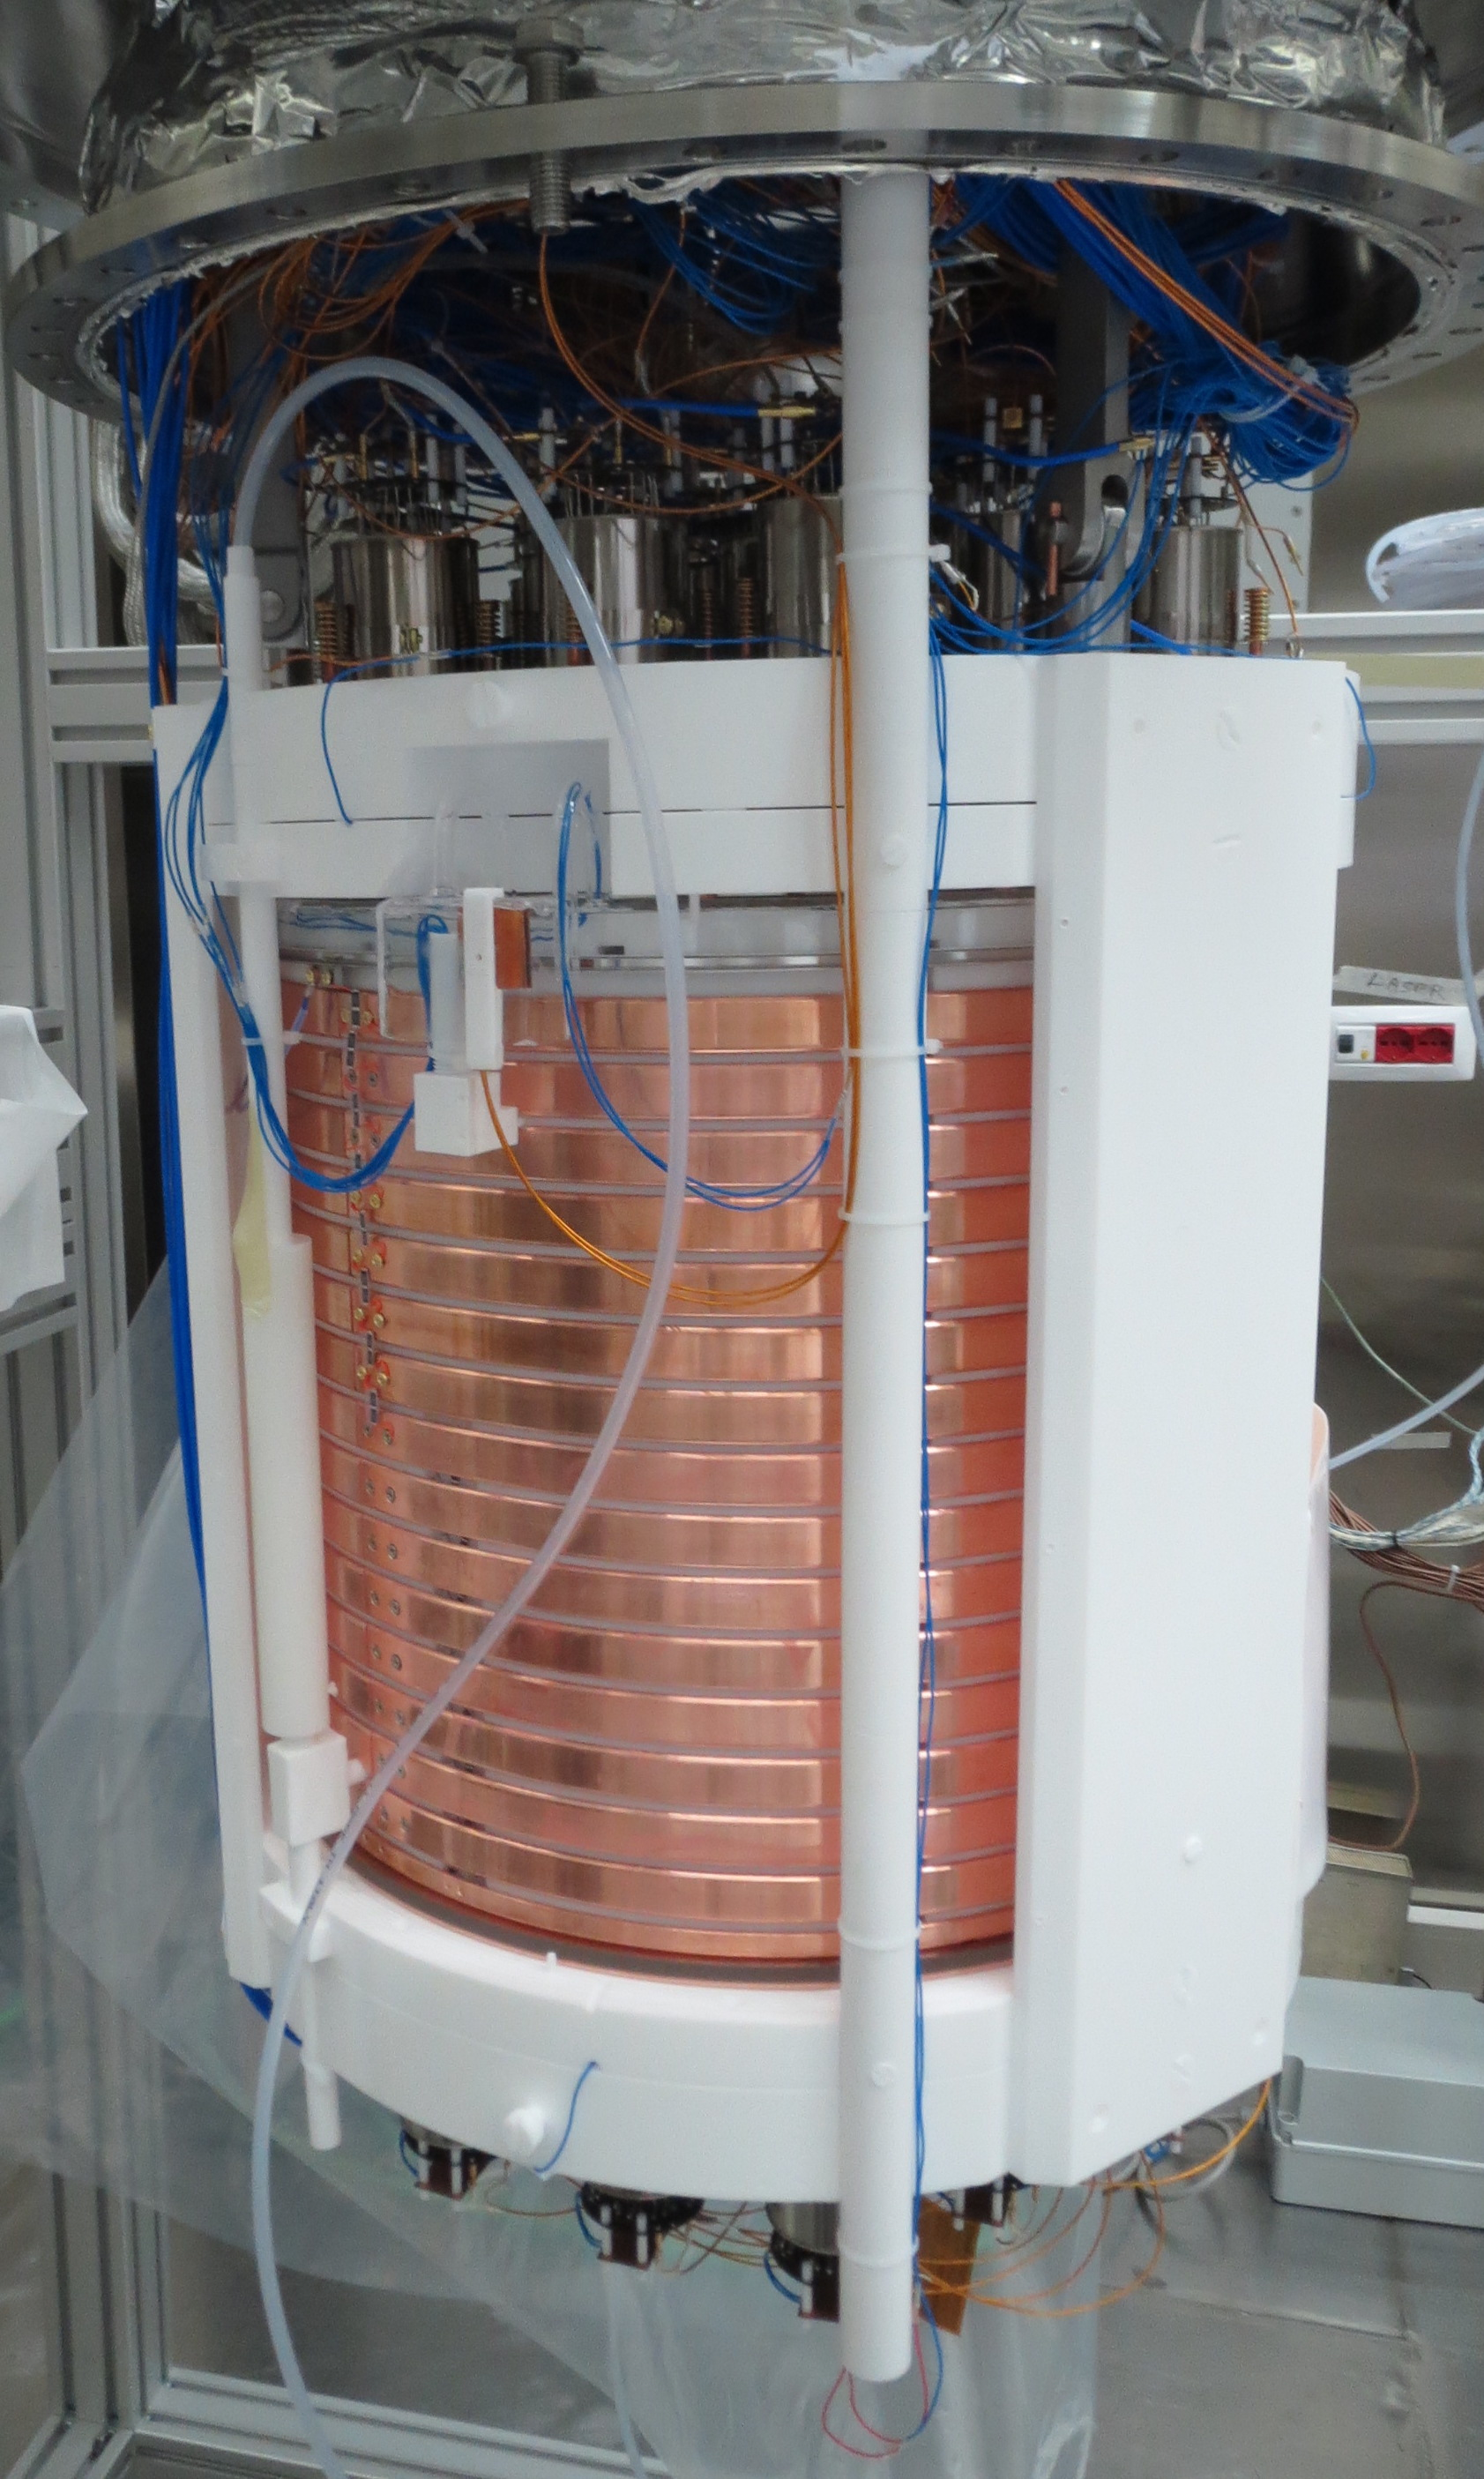
\includegraphics[height=4in]{./Figures/DSf-LArTPC.jpg}
%\hspace{0.1in}
%\includegraphics[height=4in]{./Figures/DSf-CryostatLift.jpg}
%\end{center}
%\caption{{\bf Left}: The \DSfs\ \LArTPC.  {\bf Right}: TPC cryostat being lowered into the liquid scintillator veto (\LSV) (whose top entry point is visible at the bottom of the picture), which in turn sits inside the the water Cherenkov muon veto (\WCV).}
%\label{fig:DSf-Pictures} 
%\end{figure}

Critical for the blind analysis of 532.4 live-days of UAr data was the completion of several calibration campaigns, performed either by injecting sources directly into the \LAr\ via the cryogenics and gas handling system, or by positioning sources against the \LArTPC\ cryostat with a deployment device reaching through the water tank and neutron veto~\cite{Agnes:2017ec}. These calibration campaigns have also enabled a rich set of detector-performance analyses.  For instance, an americium-beryllium neutron source was deployed for several campaigns.  \ce{^241AmBe} neutrons gave us our first direct look at \WIMP-like \NRs\ in the \LArTPC\ and neutron capture signals in the neutron veto.  Figure~\ref{fig:DSf-UArResults} (right) shows the \FNine\ response in the \LArTPC\ for \NRs\ and \ERs\ induced by neutrons and \grs, respectively, from the \ce{^241AmBe} source. It also shows the median \FNine\ response of \NRs\ as extrapolated from our independent calibration experiment, SCENE~\cite{Cao:2015ks}, and that the two measurements are in good agreement with each other.

%{\bf \ce{^{83m}Kr}:} We regularly inject \ce{^{83m}Kr} into the recirculating argon to provide a monoenergetic, low-energy \ER\ signal just above the \WIMP\ search region.  This is our primary light-yield monitor and energy calibration.  As a secondary monitor of the light-yield we monitor the measured energy of certain \gr\ lines resulting from the decay of various isotopes in the detectors materials on a run-by-run basis and ensure that the light-yield dose not fluctuate by more than \SI{1}{\percent}.

%{\bf \ce{^241AmBe} neutrons:} An americium-beryllium neutron source was deployed for several campaigns.  \ce{^241AmBe} neutrons gave us our first direct look at \WIMP-like \NRs\ in the \LArTPC\ and neutron capture signals in the neutron veto.  Figure~\ref{fig:DSf-UArResults} (right) shows the \FNine\ response in the \LArTPC\ for \NRs\ and \ERs\ induced by neutrons and \grs, respectively, from the \ce{^241AmBe} source. It also shows the median \FNine\ response of \NRs\ as extrapolated from our independent calibration experiment, SCENE~\cite{Cao:2015ks}, and that the two measurements are in good agreement with each other.  Figure~\ref{fig:DSf-AmBeCaptureSpectrum} shows the spectrum of \ce{^10B} captures in the neutron veto.  The lower energy peak at around \SI{28}{\pe} shows our efficient detection of the heavily quenched $\alpha$'s from the capture to the \ce{^7Li} ground state (\BTenNeutronCaptureGroundDecayBR\ branch, orange box), which is crucial to achieve the well over \SI{99}{\percent} neutron veto efficiency~\cite{Agnes:2016fw}.

\begin{figure}[!t]
\begin{center}
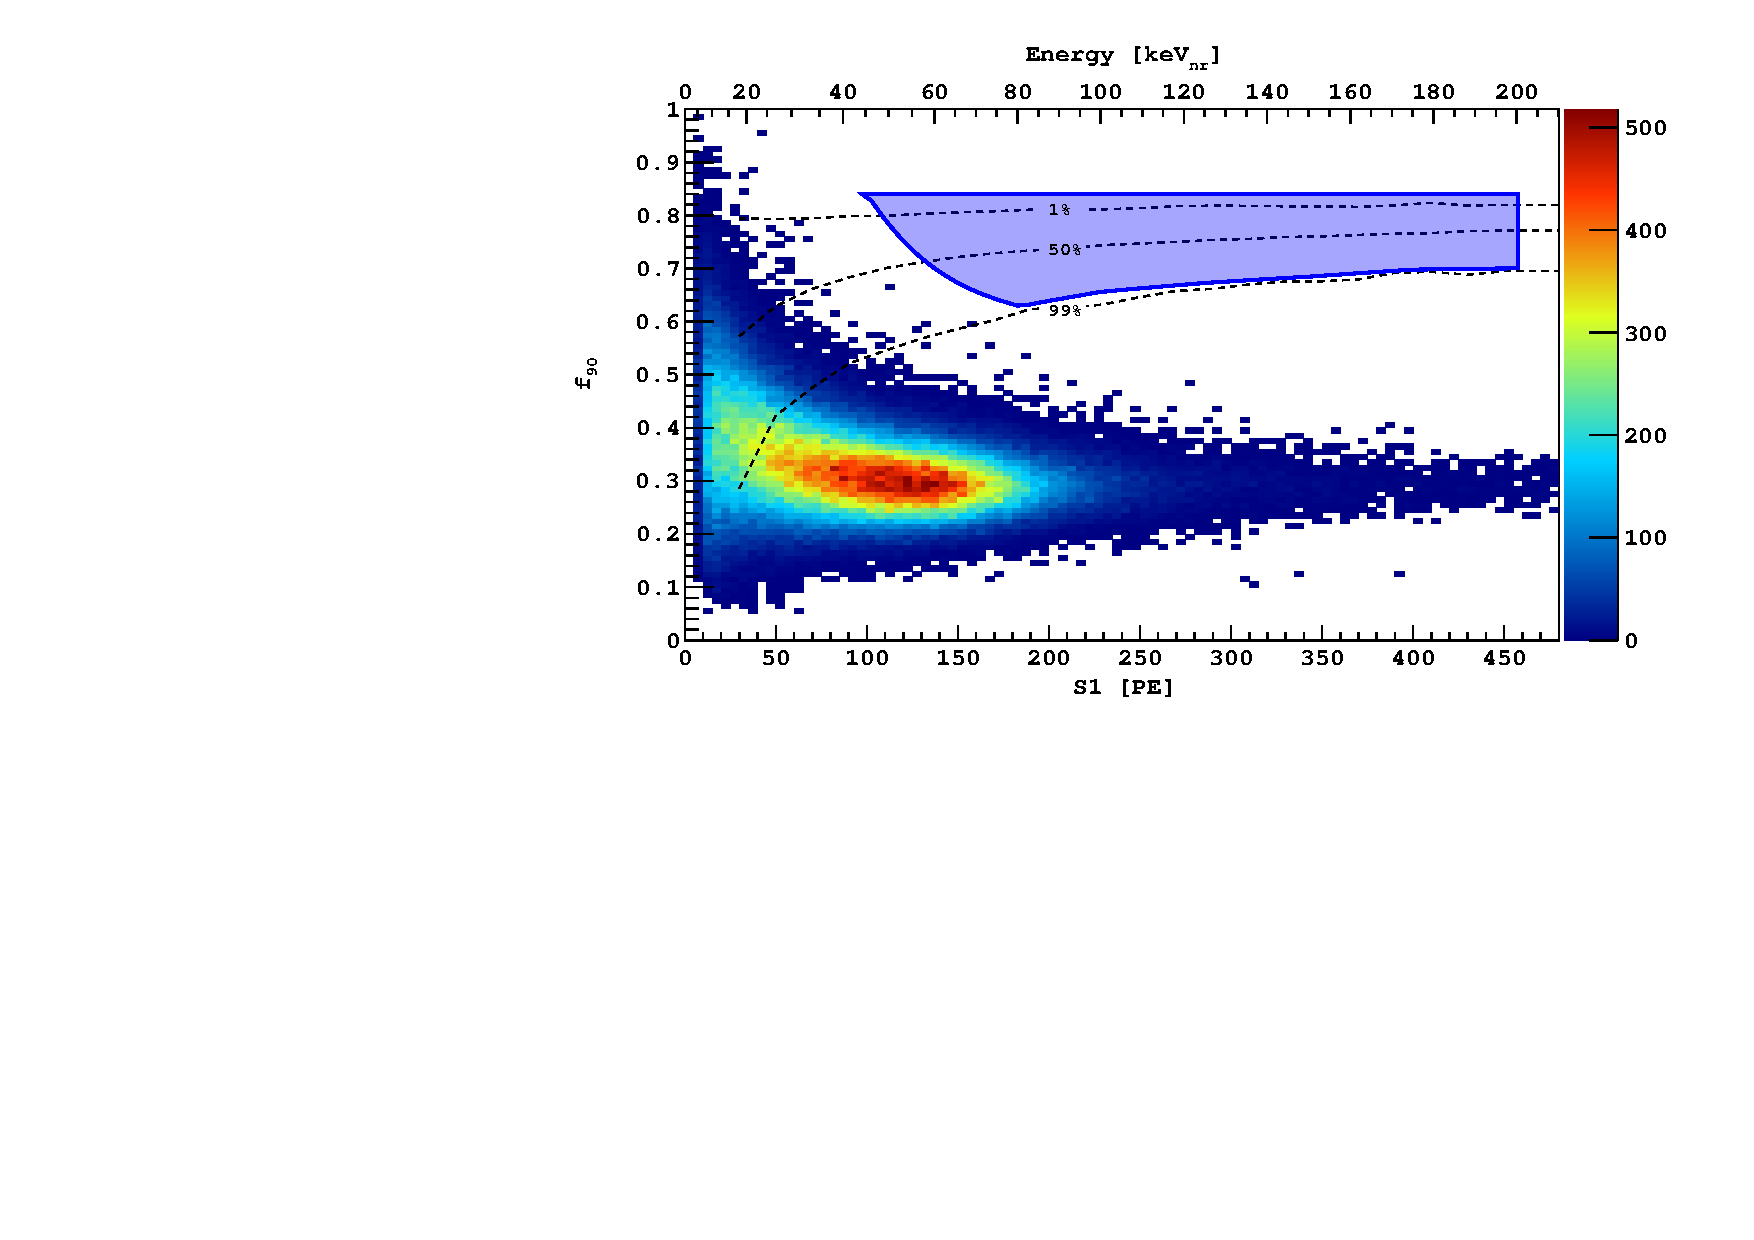
\includegraphics[width=0.525\textwidth]{./Figures/DSfHighMassSearch.pdf}
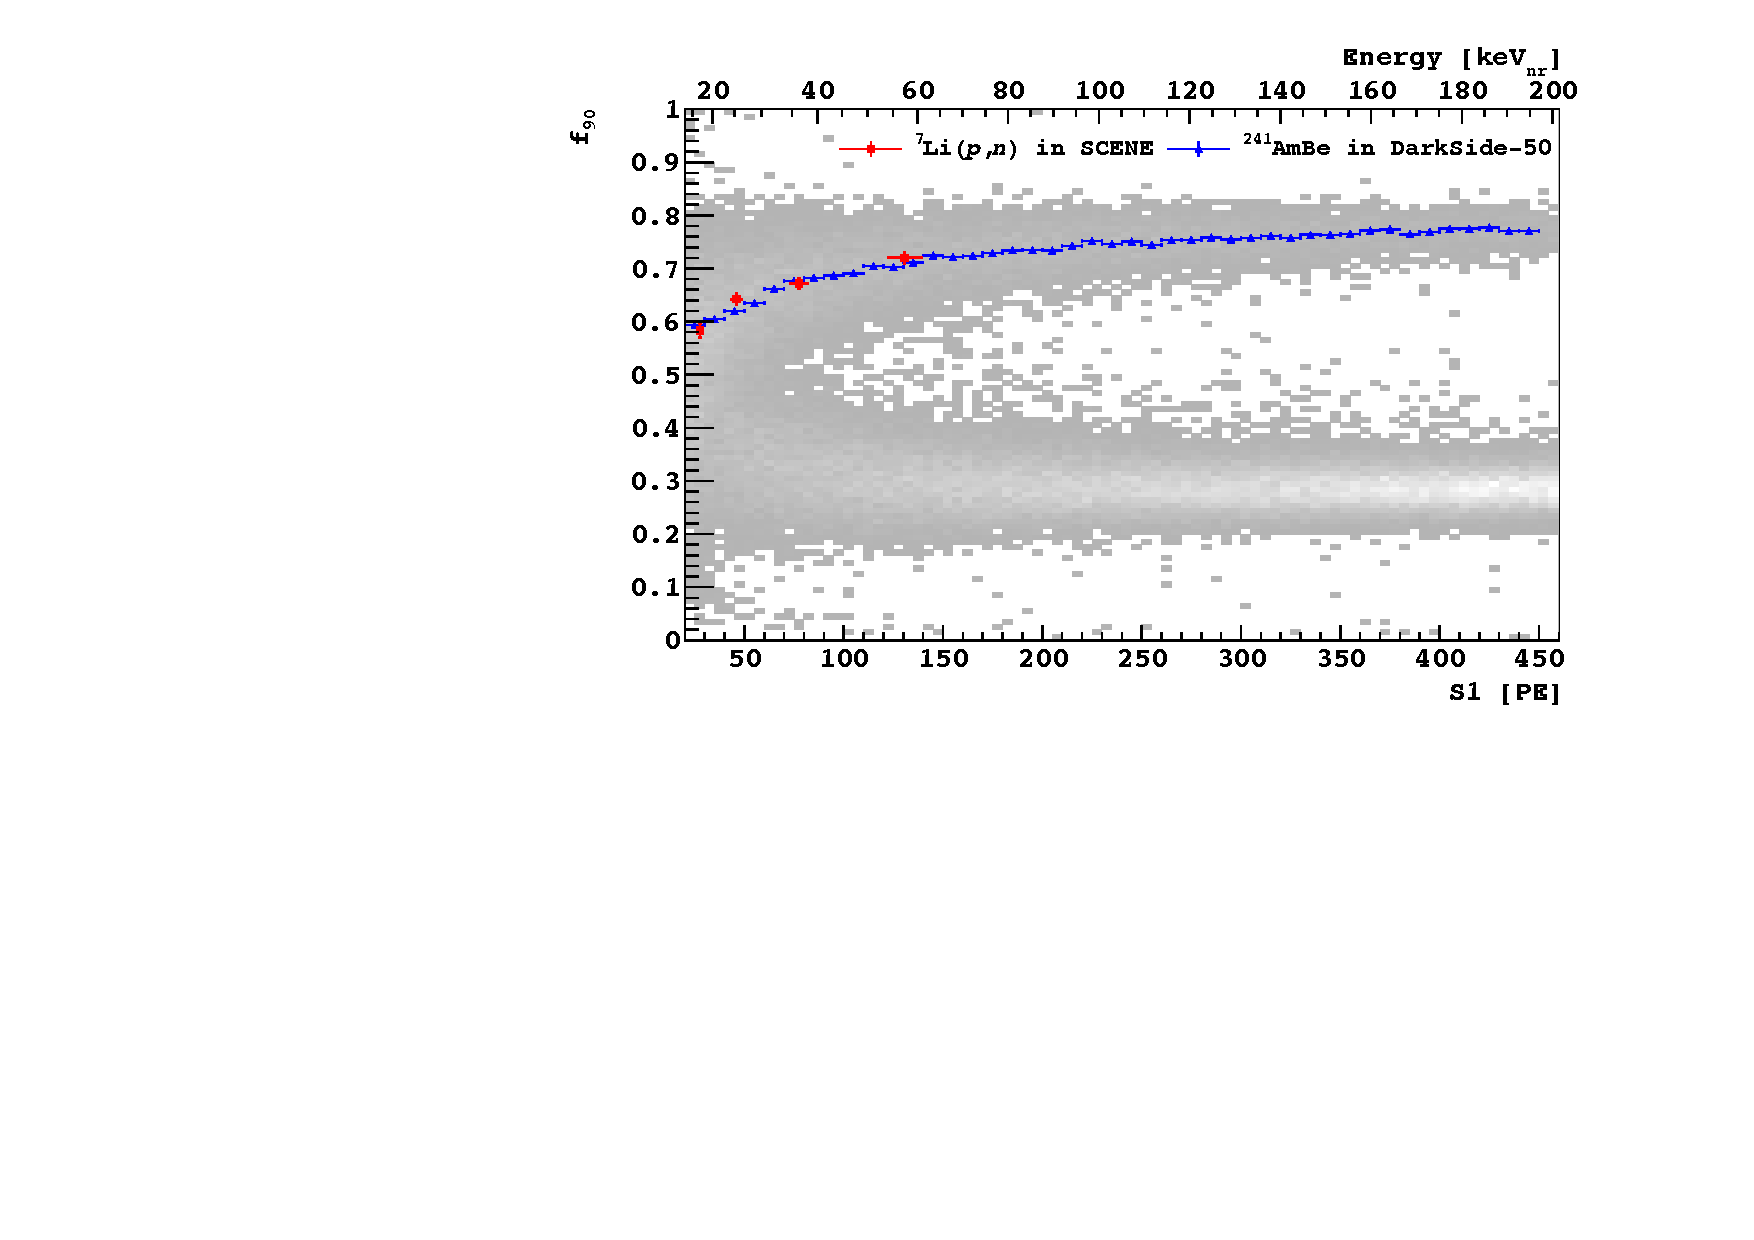
\includegraphics[width=0.455\textwidth]{./Figures/DSf-UArAmBeDMSStCut.pdf}
\end{center}
\caption{{\bf Left}: Results from a run of \DSf\ with a \UAr\ fill for a 532.4 live-days livetime.  The plot shows the distribution of events in the main pulse shape discriminant, \FNine\ (the fraction of the primary scintillation pulse in its first \WindowFNine) vs. the total integral of the primary scintillation pulse, \SOne\ (measured in photoelectrons, \si{\pe}).  The dashed lines identify the lower boundaries of nuclear-recoil signal regions having the indicated acceptances.   The shaded blue region above the blue line is the WIMP search box.  The NR energy scale relevant for \WIMP\ scattering is shown across the top axis.  {\bf Right}: \FNine\ vs.~\SOne\ distribution for \NRs\ (\WIMP-like) and \ERs\ (background) from \ce{^241AmBe} calibration data.  The scatter of events between the bands is due to $n$+$\gamma$ mixed events from the source.  Our measurements of the median of the \NR\ band are compared to those from \SCENE, which cover only the low energy range.}
\label{fig:DSf-UArResults}	
\end{figure}

%{\bf \ce{^241Am^13C} neutrons:} The neutron veto also detects  neutrons via elastic scatters from the hydrogen in the scintillator.  The high rate of coincident \grs\ in \ce{^241AmBe} prevents detection of this signal.  An americium alpha source irradiating a \ce{^13C} target through  a thin gold foil yields neutrons without exciting the final-state \ce{^16O}.  This gives neutrons with essentially no coincident high-energy \grs\ (only the \AmTwoFourGammaOneEnergy\ \grs\ from \ce{^241Am} that are stopped by a \SI{2}{\milli\meter} thick lead shield).  We produced such a source, and the \ce{^241Am^13C} data allowed us to study events in which a neutron produces a \WIMP-like signature in the \LArTPC\ either before or after scattering and/or capturing in the LSV.  We were therefore able to {\it measure} the veto efficiency for neutron-induced \NRs\ in the \LArTPC.  Using a Monte Carlo simulation to correct for the different origin and energy spectrum of neutrons from the source compared to radiogenic neutrons from detector materials, we estimated a data-driven neutron veto efficiency well above \SI{99}{\percent}.

%\begin{figure}[!t]
%\begin{center}
%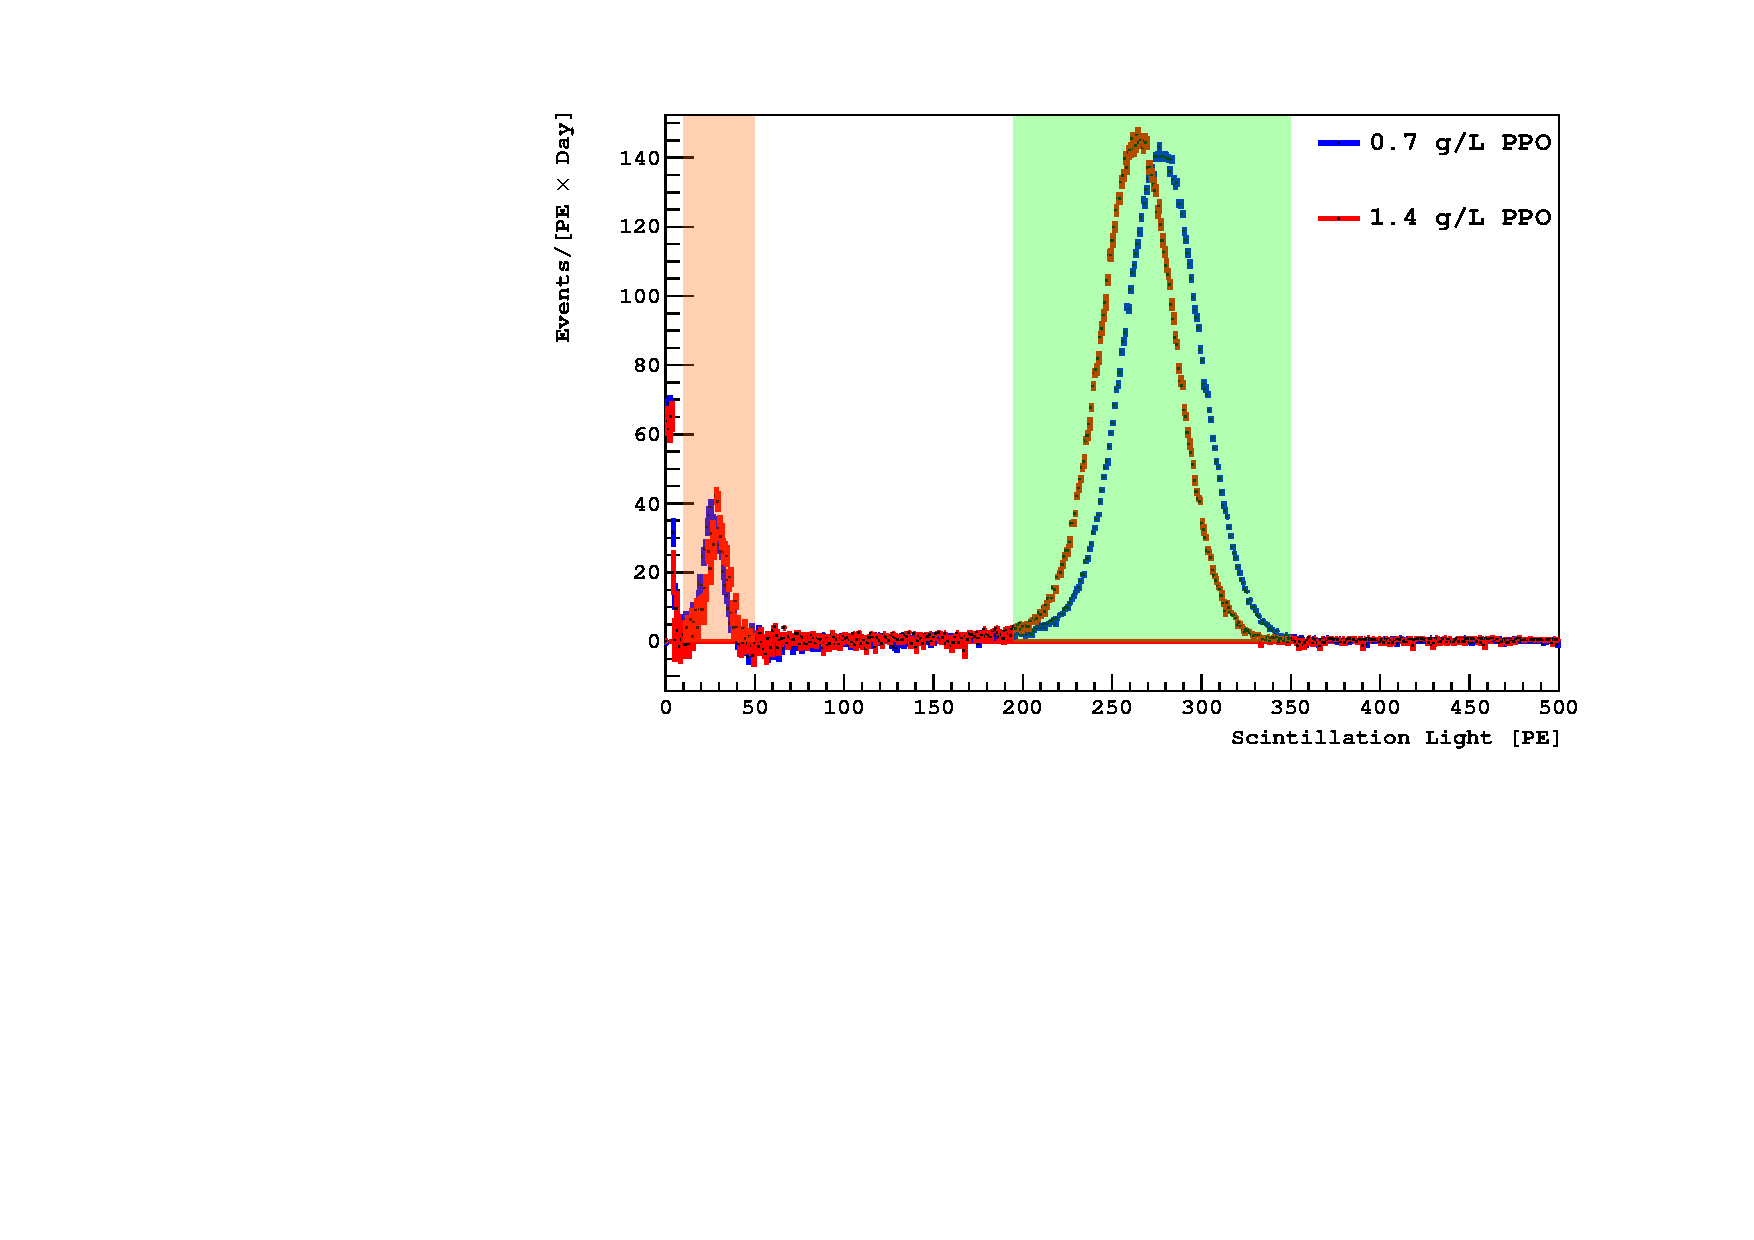
\includegraphics[width=0.8\textwidth]{./Figures/DSf-AmBeCaptureSpectrum.pdf}
%\end{center}
%\caption{Neutron-capture on \ce{^10B} in our borated-liquid-scintillator neutron veto with two versions of the scintillator cocktail.  The orange (green) box indicates the signal from the $\alpha$-only ($\alpha$+$\gamma$) final state.}
%\label{fig:DSf-AmBeCaptureSpectrum} 
%\end{figure}

The \DSs\ external calibration campaigns have provided measurements crucial for optimizing the operation of the \DSfs\ detector and extraction of its scientific results. The two major efforts that the \GADMC\ Collaboration has already undertaken are:

\begin{compactitem}

\item {\bf \SCENE:} The first measurement of the low-energy light (\SCENERecoilsLightEnergyRange) and charge (\SCENERecoilsIonizationEnergyRange) yields for \NRs\ as a function of drift field was performed in the \SCENE\ experiment~\cite{Alexander:2013ke,Cao:2015ks}, led by members of the \DSf\ collaboration. The choice of a standard drift field value of \DSfDriftField for \DSfs\ was based on the \SCENE\ results, and motivated by the need to minimize the loss of scintillation light for \NRs\ due to higher drift fields. The \NR\ energy scale and \NR\ acceptance curves used in the \DSfs\ science papers~\cite{Agnes:2015gu,Agnes:2016fz} were also determined using the \SCENE\ data. Finally, the \SCENE\ experiment gave a hint about the directional signature in the scintillation response of \SCENERecoilsEnergyMax\ \NRs.

%\begin{figure}[!tb]
%\begin{center}
%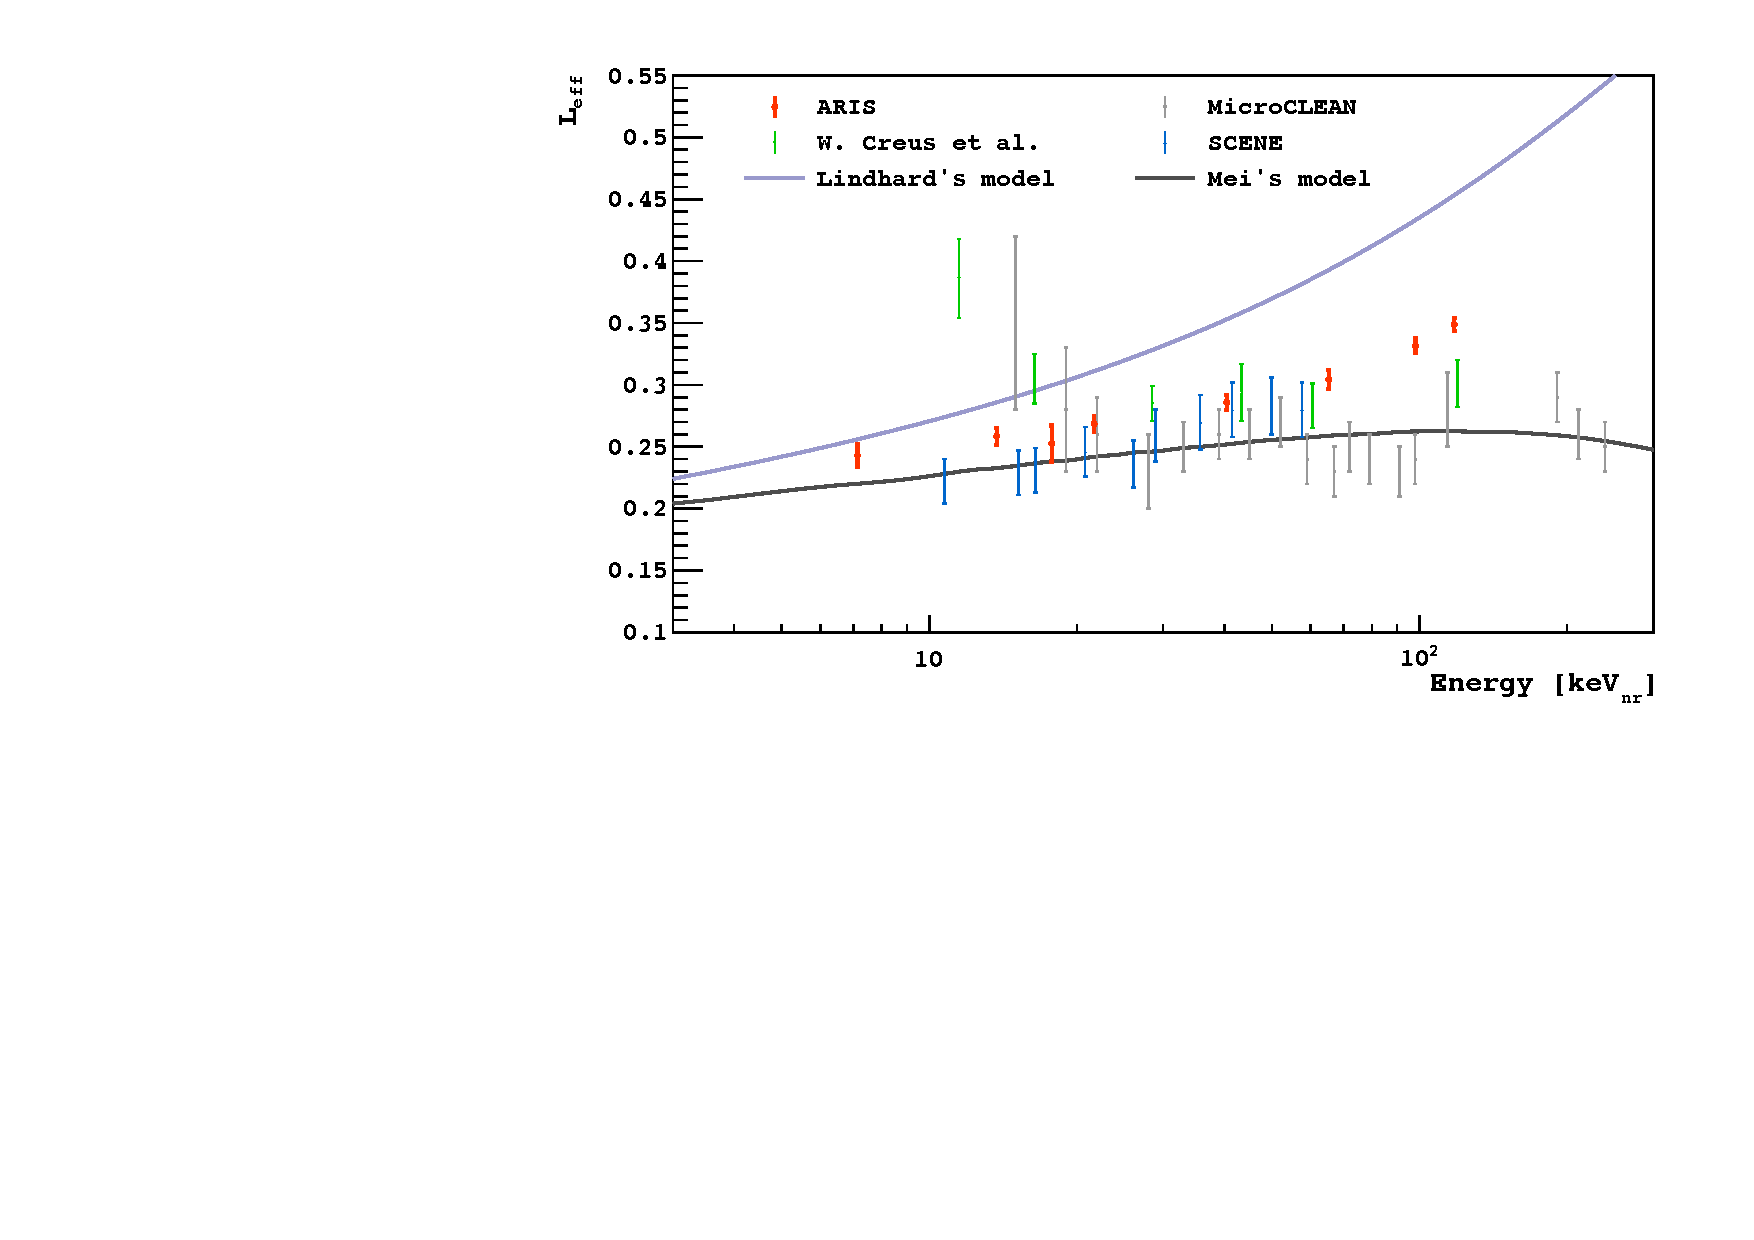
\includegraphics[width=0.8\textwidth]{./Figures/ARIS-Quenching.pdf}
%\end{center}
%\caption{\ARIS\ results for quenching of \NR\ light yield in \LAr.  The ratio of \NR/\ER\ light yield at zero field is shown vs. \NR\ energy.  This preliminary result is compared to previous measurements (see~\cite{Cao:2015ks} and references therein).  Publication of the \ARIS\ results is expected during CY~2017.}
%\label{DSf-ARIS-Leff} 
%\end{figure}

%\begin{figure}[!htb]
%\begin{center}
%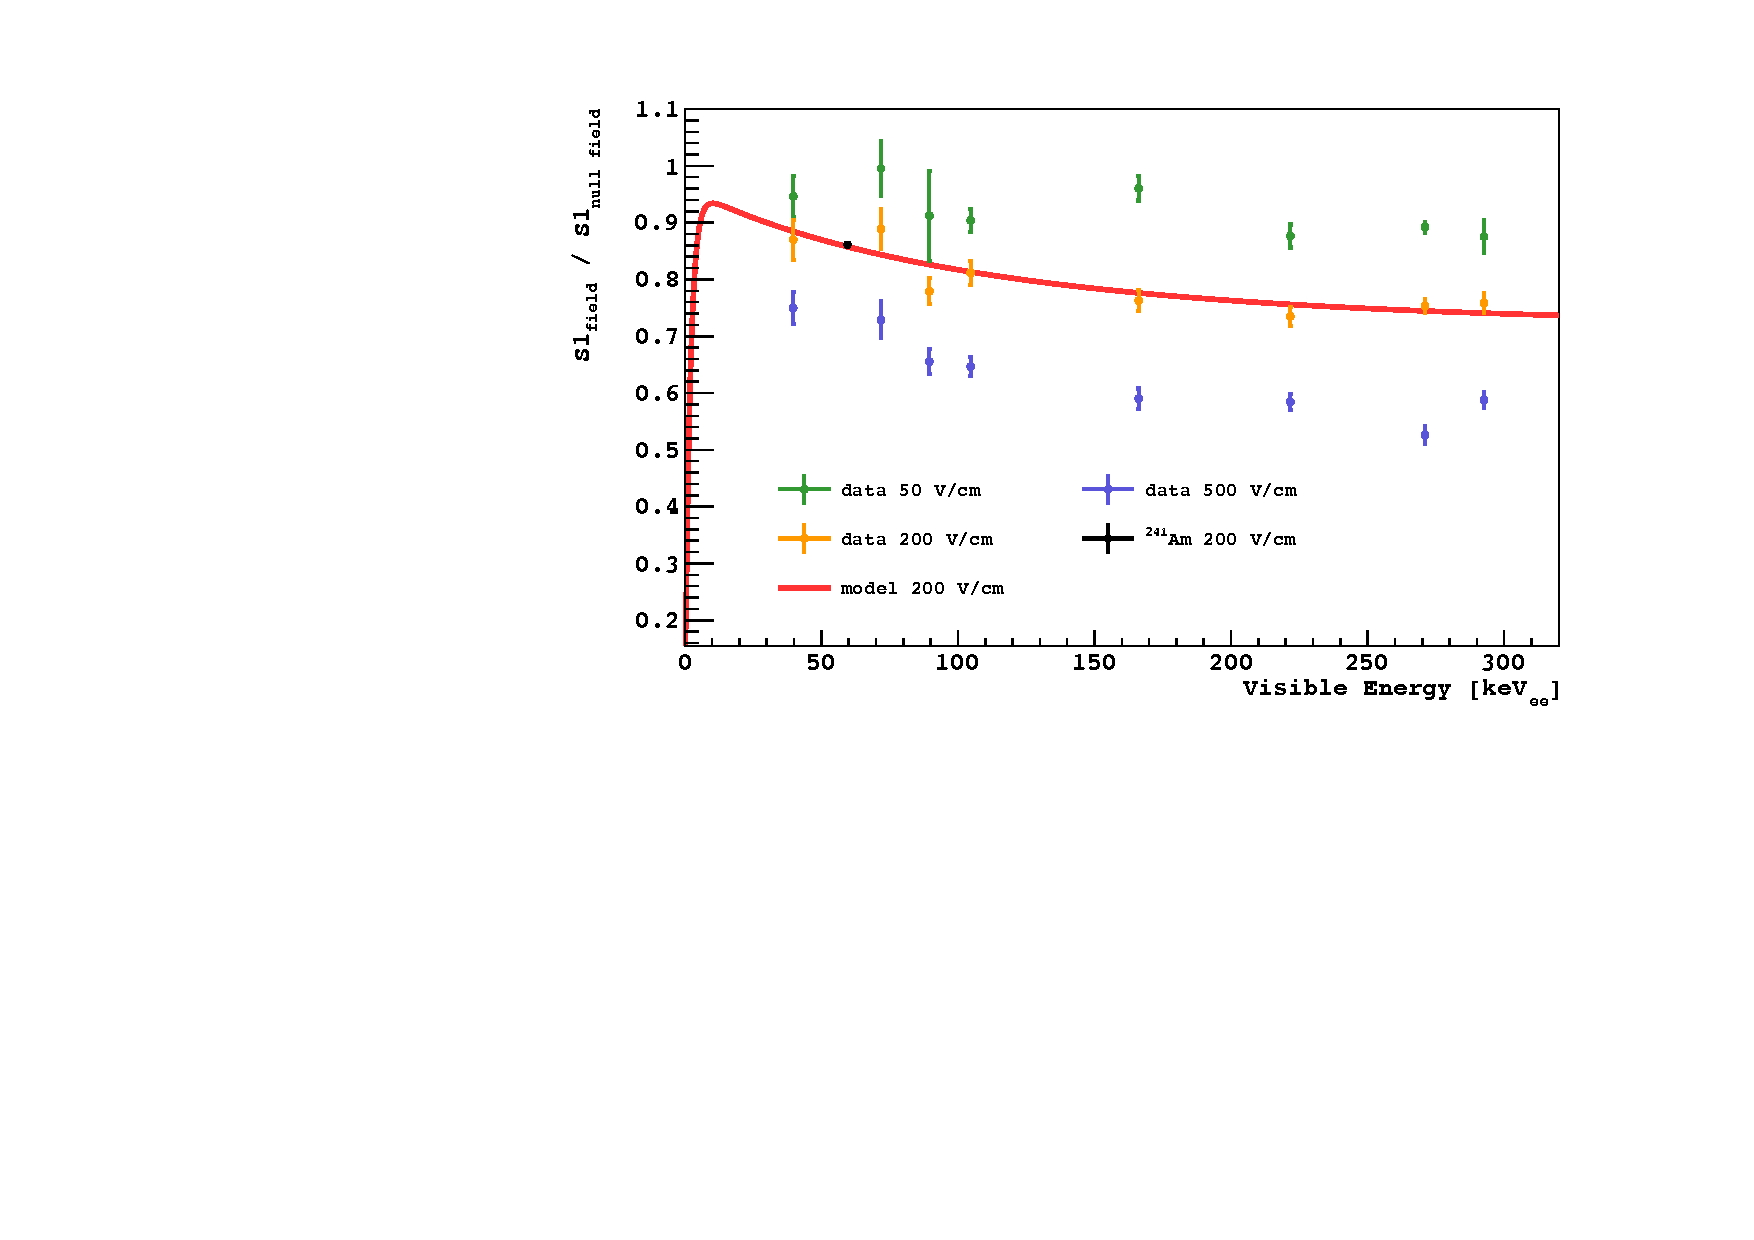
\includegraphics[width=0.49\textwidth]{./Figures/ARIS-ERfield.pdf}
%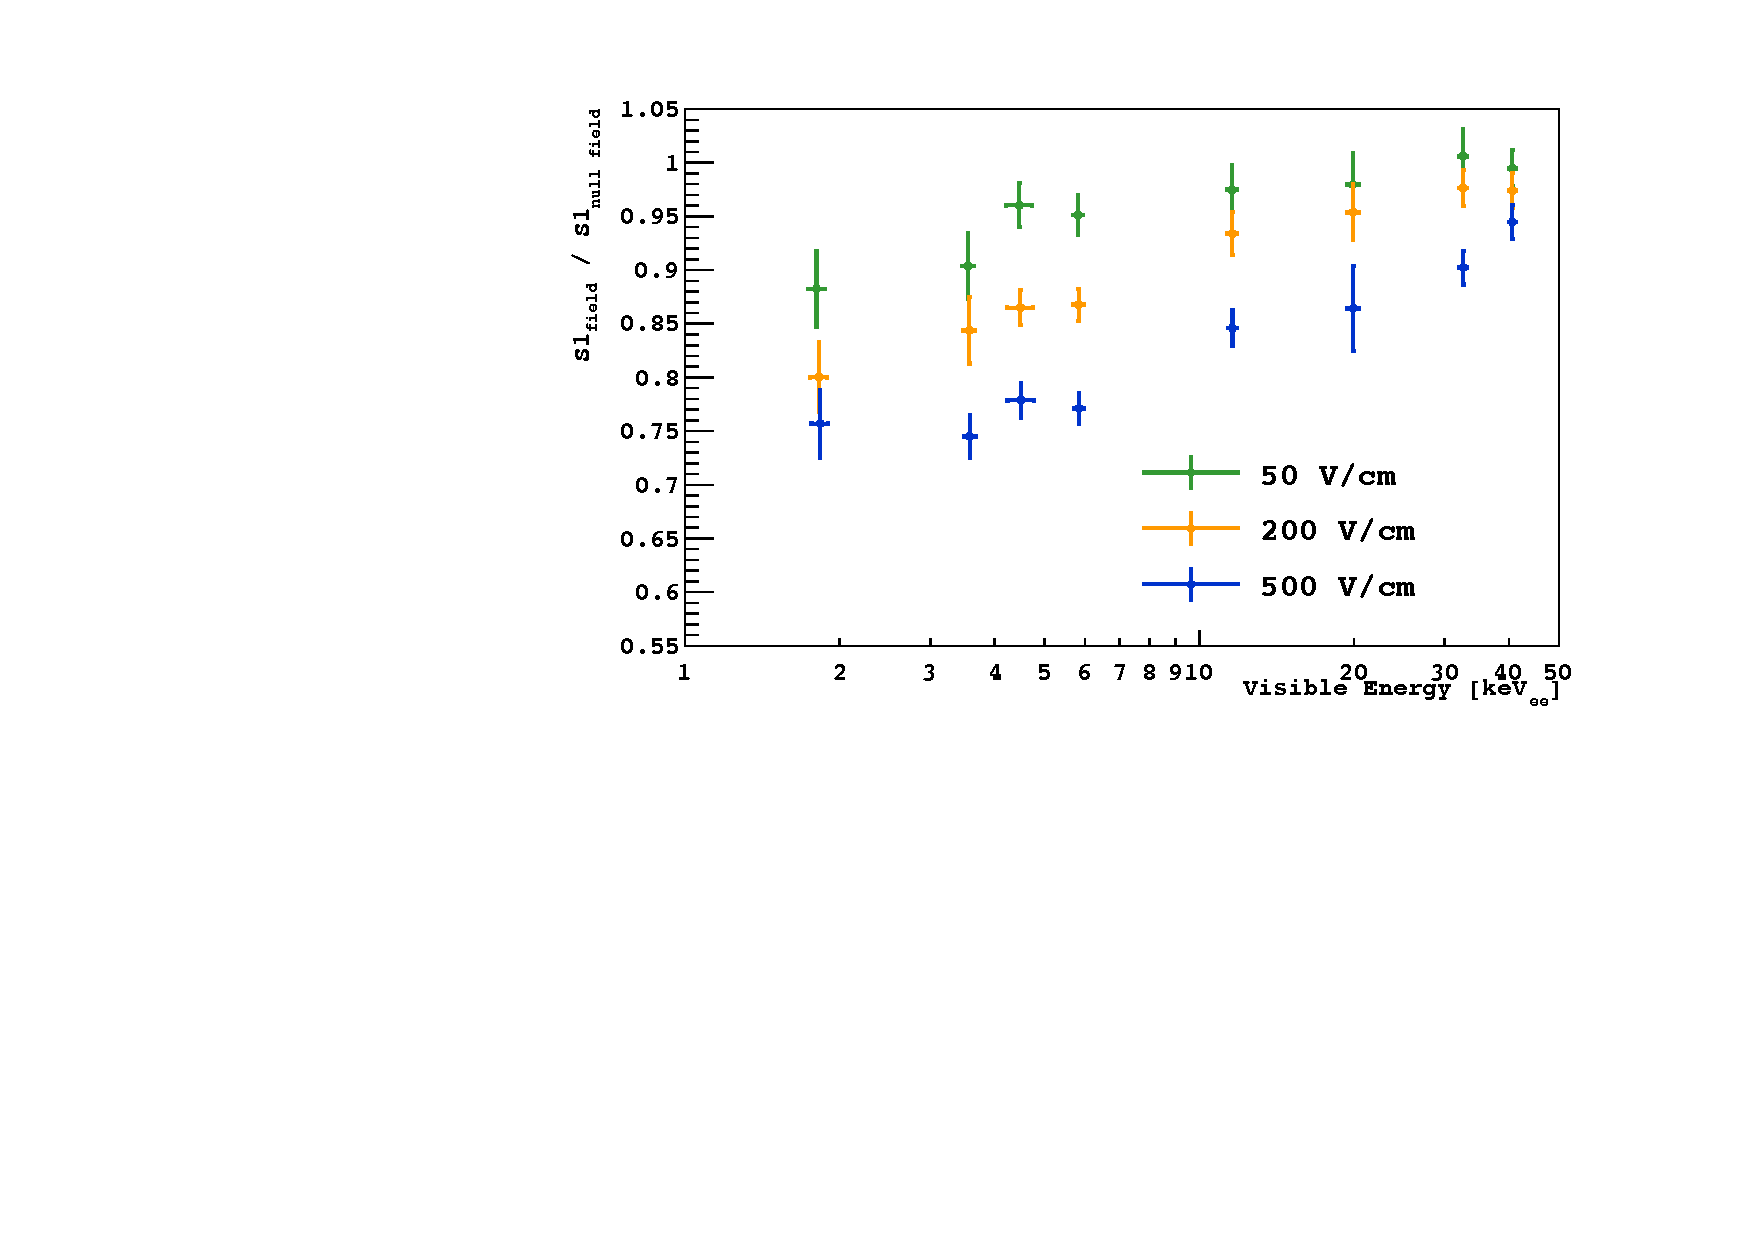
\includegraphics[width=0.49\textwidth]{./Figures/ARIS-NRfield.pdf}
%\end{center}
%\caption{{\bf Left}: Preliminary \ARIS\ results for quenching of \ER\ light yield in \LAr\ at different drift fields. The \DSkDriftField\ dataset is compared to the PARIS model tuned on \DSf\ data~\cite{Agnes:2017ug}. {\bf Right}: Preliminary \ARIS\ results for quenching of \NR\ light yield in \LAr\ at different drift fields. Publication of the \ARIS\ results is expected during CY~2017.}
%\label{DSf-ARIS-Recombination} 
%\end{figure}

\item {\bf \ARIS:} The \ARIS\ experiment also provided light yield measurements for \NRs\ as a function of the drift field, and did so with much higher precision and spanning a larger energy range (\ARISRecoilsLightEnergyRange) than \SCENE.  Additional \ARIS\ results include measurements of the recombination probability of electron-ion pairs as a function of energy and applied electric field for both \ERs\ and \NRs, and the confirmation of the light yield linearity of the \LAr\ \ER\ response. These results are important in the construction and calibration of models which predict the behavior of \LAr\ to recoiling electrons and nuclei. The Precision Argon Response Ionization and Scintillation (PARIS) model has been developed to describe the \LAr\ response inside the \DS\ \LArTPC\ detectors~\cite{Agnes:2017cz}. We plan to use \ARIS\ data to further improve the PARIS model, a crucial tool for predicting the sensitivity of future large \LAr\ detectors in the search for dark matter.

\end{compactitem}

In addition to the publications referenced above, we have published a technical paper detailing the electronics and data acquisition of the \DSfs\ veto detectors~\cite{Agnes:2016cp}, a physics paper describing the effect of low electric fields on scintillation light yield from $\alpha$'s in \LAr~\cite{Agnes:2017cl}, a technical paper describing our simulation of argon response and light detection in \DSfs~\cite{Agnes:2017cz}, a technical paper describing the calibration source deployment system~\cite{Agnes:2017ec}, a physics paper describing radiogenic neutron yield calculations for low-background experiments~\cite{Westerdale:2017vr}, a technical paper detailing the electronics, trigger and data acquisition system of the \DSfs\ \LArTPC~\cite{Agnes:2017ck}, and a physics paper describing the electroluminescence pulse shape and electron diffusion in liquid argon~\cite{Agnes:2018dt}.

%---
\subsection{Broader Impact}
\label{sec:PreviousResults-BroaderImpact}

Since its inception in 2009, the \NSF-funded \DSs\ program has had significant broader impacts in the areas of education and outreach, and the program's scientific developments have impacted industry and a variety of basic research fields.

Through 2012, the collaboration offered a unique multi-cultural summer program that brought together high-school students from Italy and South Dakota for underground-physics-related instruction and activities at Princeton, \LNGS, and Sanford Lab.  The program, the Gran Sasso-Princeton-South Dakota Summer School, benefited several hundred students.

Most groups in the collaboration have given undergraduate students the opportunity to contribute to the research effort in various ways.  These include formal education (junior and senior theses at Princeton, Houston, Augustana, Hawaii, UCLA, Temple, and elsewhere; TURF-CREWS projects at Temple, etc.) as well as informal activities, such as lectures to large General Physics classes (UCLA, others), Physics Clubs (Temple, others),  undergraduate seminars, and the like. The Augustana PI regularly visits high school physics classes in South Dakota to talk about underground physics, contacting around \num{300}~students each year.  The Hawaii PI and students act annually as section leaders in the ``Expanding your horizons'' science workshop for middle school girls.  The Temple PI has given invited informal talks to local astronomy clubs and to a local retirement community. The UC Davis PI and group members annually contribute to a hands-on summer school for undergraduate and graduate students from various disciplines. Princeton PI Cristiano Galbiati visited over twenty schools in the Sulcis-Iglesiente district of Italy, near the site of the \Aria\ cryogenic distillation plant discussed below.  These visits presented the research program of the \GADMC\ collaboration and the plans for the \Aria\ project to more than \num{1000} students.

Technologies developed for the \DSs\ program have had or may develop significant impacts on industry and other branches of science.  A non-exhaustive list includes:

\begin{compactitem}

\item In the course of our \UAr\ extraction from natural gas wells, significant amounts of \ce{^4He} were discovered in the gas stream.  \ce{^4He} is essential in many branches of science. It is a scarce, non-renewable resource which is rapidly growing in cost and scarcity.  Throughout the operation of the  \DSfs\ \UAr\ extraction plant at the Kinder Morgan Doe Canyon \ce{CO_2} facility near Cortez in southwestern Colorado, we measured and kept records of the content of \ce{^4He}.  We demonstrated to Kinder Morgan the presence of a sustained and commercially exploitable fraction of helium in their gas stream.  This result led to the start of the first ever commercial enterprise to extract helium from a \ce{CO_2} stream.  Air Products built a helium production plant treating the entire Kinder Morgan Cortez \ce{CO_2} stream, which started production in \UraniaHeStartDate\ and presently supplies \ce{^4He} equivalent to \UraniaHeNationalReserveFractionEquivalentRate\ of the declining production from the US National Helium Reservoir.  The discovery of helium in Cortez performed by the \GADMC\ Collaboration enabled the provision of major quantities of this crucial resource, which is regularly shipped to serve research laboratories and industries across the US.

\item The \UAr\ itself is finding applications in ultra-low-level counting applications such as nonproliferation and clandestine nuclear test detection, groundwater aging studies, and other areas.

\item Princeton PI Cristiano Galbiati invented the cryogenic distillation plant ``\Aria'' for active isotopic purification of \UAr\ for \DSks\ and larger projects.  \Aria\ was further developed by \DSfs\ collaborators.  Funded by the Italian Government and Regione Autonoma della Sardegna, the first \Aria\ column will be the tallest plant in the world at \AriaSeruciHeight\ in height.  Installation inside a mine shaft in Sardinia will start in 2019. Thanks to its high mass resolution and throughput, \Aria\ will have the ability to increase the world-wide availability (and lower the cost) of rare stable isotopes important to industry, science, and medicine, including \ce{^18O}, \ce{^13C}, \ce{^15N}, and others.

\item Princeton PI Cristiano Galbiati proposed and founded the Nuova Officina Assergi (\NOA), a modern clean-room facility for the assembly of silicon devices that will be located at \LNGS\ and first used to build the \SiPM-based cryogenic photodetectors of \DSks.  \NOA\ is funded by Regione Abruzzo and the Italian Government.  This development was made possible by the early (2014) decision of the \GADMC\ collaboration to abandon the development of \PMTs\ and to focus the \DSs\ R\&D on \SiPMs and the ensuing success obtained by the Collaboration in that development.  As a direct result of this early focus, \DSs\ researchers produced many leading results on the utilization of \SiPMs\ as cryogenic photosensors.  In particular, we demonstrated the operation of large (tens of \si{\square\cm}) single-channel cryogenic photosensors with single photoelectron sensitivity, defeating the noise induced by the very large capacitance of \SiPMs\ arrays.  Today, these large photosensors allow us not only to replace \PMTs\ for \DSks, but also to surpass their technical performance in every metric.  Our \SiPM-based cryogenic photosensors maintain the excellent photon detection efficiency and resolution of \SiPMs, superior to those of \PMTs, and also possess, at cryogenic temperature, a dark noise rate lower than \PMTs~\cite{DIncecco:2018hy}.

\item Other ultra-clean technical methods developed for \DSfs\ extend the reach of important existing industrial processes ({\it e.g.}, precision cleaning) or offer new possibilities for industrial processing (radon-suppressed clean rooms).

\item The application of the \LArTPC\ concept, in conjunction with the use of \SiPMs, to build higher-resolution \PET\ scanners has been proposed and is under development at Princeton.

\end{compactitem}

The maintenance and further development of all these techniques will continue to be essential for the \GADMC\ effort in the \DSks\ era and beyond.